\documentclass[11pt, letterpaper]{article}
\usepackage[margin=2cm]{geometry}
\usepackage{fourier}
\usepackage[T1]{fontenc}
\usepackage[utf8]{inputenc}
\usepackage{amsmath}
\usepackage{bookmark}
\usepackage{hyperref}
\usepackage{booktabs}
\usepackage{multicol, caption}
\newenvironment{Figure}
  {\par\medskip\noindent\minipage{\linewidth}}
  {\endminipage\par\medskip}
\usepackage{cite}
\usepackage{graphicx}
\usepackage{wrapfig}
\providecommand{\tightlist}{%
  \setlength{\itemsep}{0pt}\setlength{\parskip}{0pt}
}
\setlength{\columnsep}{1cm}
\setcounter{secnumdepth}{-\maxdimen}
\title{Fake Face Detection and Fairness}

\author{
  Alex Kyllo
  \and
  John Wyman
  \and
  Will Thomas
}

\begin{document}

\maketitle

\begin{abstract}
  In this study we investigate whether it is still feasible to automatically
  discern AI-generated human face images from genuine photographic ones, by
  training a convolutional neural network on a labeled dataset of 70,000 real
  and 70,000 fake face images. We use the fake face classification problem to
  further explore the topic of model fairness, by evaluating the model's
  performance across age, gender and race groups on a demographically labeled
  face dataset. To achieve this, we propose a method of utilizing an autoencoder
  network to translate demographically labeled real face images into an
  approximation of their latent space code representations and then reconstruct
  them back into images, creating a dataset of matching fake face images with
  the same demographic labels. This allows us to assess whether our fake face
  detection model works equally well for human faces of different age, gender
  and race groups, or whether it even generalizes to a dataset that is
  demographically diverse and balanced.
\end{abstract}

\begin{multicols}{2}
  \section{Introduction}

  Generative Adversarial Networks (GANs) have created the ability to encode
  photographic images into a latent space representation and automatically
  generate many images that can appear to be genuine photographs, to the human
  eye. NVIDIA's StyleGAN\cite{stylegan} model, trained on a dataset of human
  face images, is capable of generating extremely photo-realistic images of
  people who do not exist. StyleGAN is an example of a generative adversarial
  network (GAN), a type of network that consists of two models, a
  \emph{generator}, which learns a data distribution from a training set and
  draws from it, and a \emph{discriminator}, which learns to estimate the
  probability that a sample came from the training data or from the generator
  \cite{goodfellow2014generative}.

  The application of GANs to generating realistic human faces has garnered much
  media attention in recent years. The well-known website
  \href{https://thispersondoesnotexist.com/}{This Person Does Not Exist} serves
  random, high-resolution fake face images drawn from StyleGAN. Many models have
  been created for exploring the latent space of StyleGAN to discover vectors
  that correspond to semantic directions in which the latent codes can be
  perturbed in order to make semantic edits to human face photos, such as making
  the face look older vs. younger, more masculine vs. more feminine
  \cite{shen2020interpreting}, or thinner vs. heavier
  \cite{pinnimty2020transforming}. The popular mobile application FaceApp
  utilizes this method to allow users to transform images of themselves in this
  manner and share them on social media for humor. Two different people's face
  images can also be blended together by encoding both images and interpolating
  some point between them in the latent space, which can be used for applications
  like visualizing what a couple's children might look like, a concept that
  has been implemented in the project
  \href{https://medium.com/swlh/familygan-generating-a-childs-face-using-his-parents-394d8face6a4}{FamilyGAN}.

  It is also easy to imagine nefarious applications of fake face generation,
  some of which have already been realized, such as swapping faces of
  celebrities onto pornographic actors or falsifying speeches by political
  leaders \cite{nguyen2020deep}. Because such applications of this technology
  can unfairly damage people's reputations and erode trust in society, there is
  a public interest in retaining the ability to effectively discern real human
  face images and video from fake ones and detect "deep fake" tampering, which
  requires training more deep learning models to distinguish them.

  A problem with the available open datasets of human faces used in
  training deep learning models, is bias in the demographic
  composition of the pictured individuals. The machine learning
  community has recently been struggling with the issue of model
  fairness--it is important that models perform equitably for users
  and data subjects of different backgrounds, and also very difficult
  to enumerate and quantify the sources of bias in training data that
  can contribute to biased model performance.

  The FairFace\cite{karkkainen2019fairface} study introduced a new
  dataset of human face images collected from public datasets with
  manually verified, crowdsourced age, gender and race labels. The
  FairFace paper demonstrates that because existing public datasets of
  human faces contain a majority of white faces, models trained on
  them fail to generalize well to datasets where more non-white faces
  are present. We suspected that this might also be the case for the
  70k real and fake faces dataset that we utilized for model training,
  and sought to test this by evaluating it on a demographically
  labeled dataset.

  While the FairFace dataset provides real human face images that can
  be used to assess disparities in a fake face detector's true
  negative and false positive rates, a second, similarly labeled
  dataset of fake face images is needed to compute true positive and
  false negative rates for specific age, gender and race groups. To
  address this gap, we investigated methods for ``falsifying'' a real
  face image by autoencoding it via the StyleGAN latent space. A
  research team at Tel Aviv University recently developed a novel
  encoder network\cite{richardson2020encoding} called
  \emph{pixel2style2pixel}, that is capable of approximately
  reconstructing StyleGAN's latent code representation of a face image
  and then decoding it back into an image. This yields a fake face
  output image that very closely resembles the real face input image,
  implying that the original demographic labels would remain valid,
  and giving us a dataset of matching real and fake faces for
  scoring our models and calculating classifier fairness metrics.

  \section{Methods}

  \subsection{Data Preprocessing and Augmentation}

  We tested several methods for preprocessing and augmenting the image data
  before feeding it into the CNN model.

  \begin{itemize}
    \tightlist
  \item 3-color (RGB) images vs. grayscale
  \item Pre-cropping and centering faces using pre-trained face
    detection models
  \item Random horizontal flips, rotations, and shears
  \end{itemize}

  Before training our CNN models we pre-cropped the images to center
  and align the faces with eyes, nose and mouth level. We utilized two
  different pre-trained face detection models. The first model we used
  was the Multi-Task Cascaded Convolutional Neural Network (MTCNN)
  \cite{Zhang_2016}. Later, we switched to utilizing the Dlib package
  implementation of the Shape Predictor 68 Face Landmarks model
  \cite{SAGONAS20163} because the \emph{pixel2style2pixel} model was
  trained on face images that were aligned with this model and expects
  such as input.

  \subsection{Model Training}

  To solve the binary classification task of distinguishing between
  real and fake human face images, we trained several variations of
  deep Convolutional Neural Networks (CNN), varying the number of
  convolution layers as well as several model hyperparameters and
  image preprocessing steps.

  Our intial baseline model was a CNN with three convolution layers
  using a 3x3 element kernel. We trained it on grayscale images from
  the 70k fair and fake faces dataset, cropped using MTCNN, with no
  image augmentations applied. The baseline model's learning curves
  over training 20 epochs are pictured in Figure
  \ref{learning-curve-baseline}.

  \begin{Figure}
    \centering
    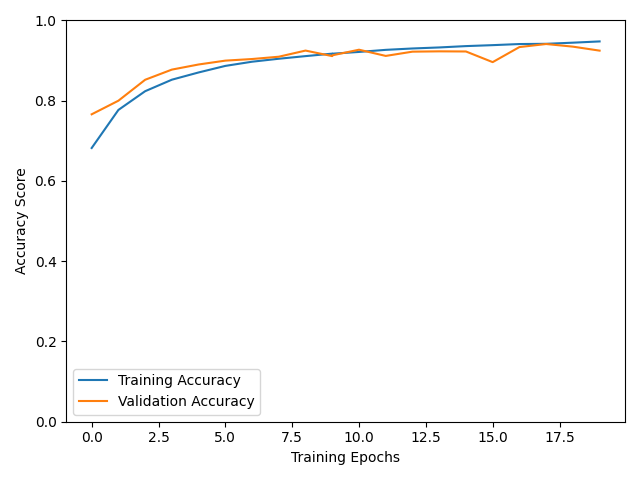
\includegraphics[width=1.0\textwidth]{figures/learning-curve-baseline-cropped-grayscale-noaug.png}
    \captionof{figure}{Learning curve for baseline model trained on fake faces grayscale images}
    \label{learning-curve-baseline}
  \end{Figure}

  Figure \ref{learning-curve-vgg10-combined} and Figure
  \ref{learning-curve-vgg10-rgb-combined} depict the learning curves
  for our best VGG-10 model, trained on the combined dataset in
  grayscale and RGB, respectively. Using RGB color images did not appear to offer
  a significant benefit, as both models were able to exceed 98\% validation accuracy
  within fewer than 20 training epochs.

  \begin{Figure}
    \centering
    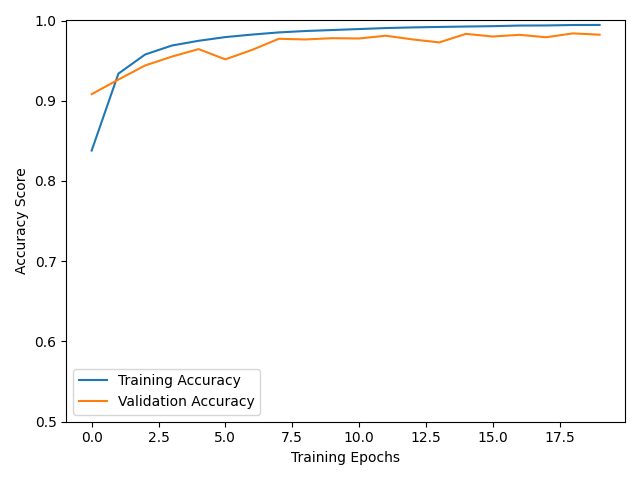
\includegraphics[width=1.0\textwidth]{figures/learning-curve-vgg10-dlib-hflip-combined-125-0001.png}
    \captionof{figure}{Learning curve for VGG-10 model trained on combined grayscale images}
    \label{learning-curve-vgg10-combined}
  \end{Figure}

  \begin{Figure}
    \centering
    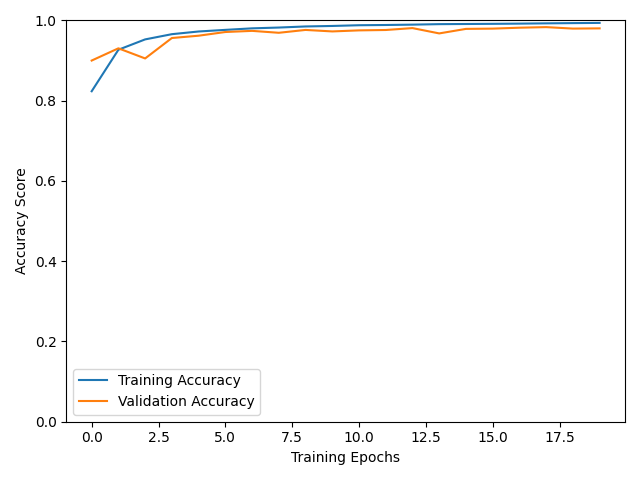
\includegraphics[width=1.0\textwidth]{figures/learning-curve-vgg10-dlib-hflip-rgb-combined-125-0001.png}
    \captionof{figure}{Learning curve for VGG-10 model trained on combined RGB images}
    \label{learning-curve-vgg10-rgb-combined}
  \end{Figure}


  \subsection{Model Serving}

  TODO: Details and screenshots of web application here

  \subsection{Model Explainability}

  TODO: Explanation and screenshot of eli5 highlighted image, possibly CNN
  activation map

  \subsection{Model Evaluation}

  Our primary metric for performance assessment during training and
  model selection was validation set accuracy, because the balanced
  classes of the input dataset made accuracy straightforward to
  interpret. For final model performance on out-of-sample test data,
  we report performance using F1 score, precision score and recall
  score in addition to accuracy score, to communicate how well the
  model performed across a variety of standard binary classifier
  metrics.

  For fairness metrics, we selected two standard binary classifier
  metrics to evaluate our classifier on: disparate impact ratio, given
  by the ratio of the rate of positive predictions for the
  unprivileged class to that of the privileged class
  \cite{fairMLHealth}, given by:

  $$\frac{P(\hat{y}|unprivileged)}{P(\hat{y}|privileged)}$$

  and average odds difference, given by:

  $$\frac{(FPR_{unpriv} - FPR_{priv}) + (TPR_{unpriv} - TPR_{priv})}{2}$$

  for the following binary group definitions taken from the FairFace
  labels:

  \begin{enumerate}
    \tightlist
  \item Gender = ``male'' vs Gender = ``female''
  \item Race = ``white'' vs all other races
  \item Race = ``black'' vs all other races
  \item Age = ``0-2'' vs all other ages
  \item Age = ``3-9'' vs all other ages
  \item Age = ``more than 70'' vs all other ages
  \end{enumerate}

  We examine the model fairness for children and senior citizens as a recent
  study \cite{9156262} found that the popular face recognition model Face++
  disproportionately fails to recognize children's faces in images collected
  from social media.

  \section{Results}

  We determined that the fake face classification task is
  still achievable with a relatively simple CNN model, but that model also
  failed to generalize to the unseen FairFace dataset.

  \subsection{Preprocessing Results}

  We utilized two pre-trained face recognition models to locate the human face
  in the image, align it so that the eyes, nose and mouth are level and
  centered, and crop to a margin around the face. Because these preprocessing
  models are themselves probabilistic machine learning models, they sometimes
  fail to recognize a human face at all (false negative) or incorrectly
  recognize some other object as a human face (false positive). We examined the
  images for which face detection failed.

  The Dlib frontal face detector method mistook several objects including a logo
  and a necklace for human faces (Figure \ref{falsepos}), while the MTCNN face
  detector method failed to identify several faces with brightly colored hair or
  wigs and heavy makeup as faces (Figure \ref{falseneg})

  \begin{Figure}
    \centering
    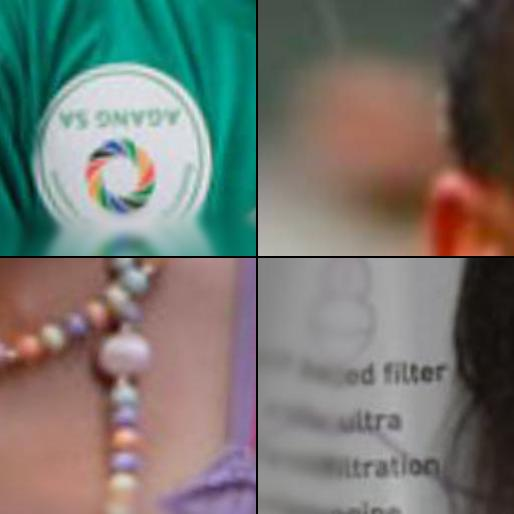
\includegraphics[width=0.7\textwidth]{figures/false-positives.jpg}
    \captionof{figure}{Sample of false positives cropped by Dlib.}
    \label{falsepos}
  \end{Figure}

  \begin{Figure}
    \centering
    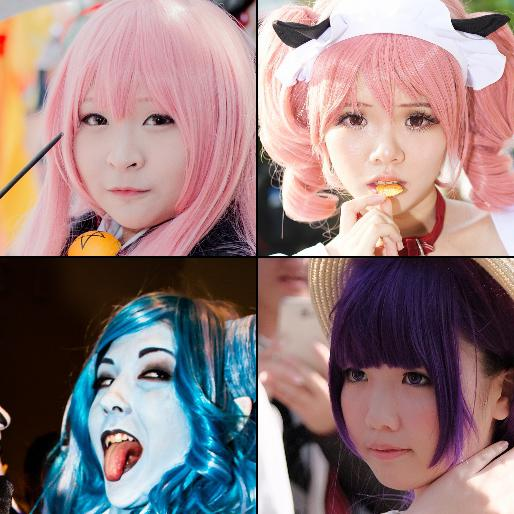
\includegraphics[width=0.7\textwidth]{figures/false-negatives.jpg}
    \captionof{figure}{Sample of false negatives that MTCNN failed to crop.}
    \label{falseneg}
  \end{Figure}

  By applying the pixel2style2pixel encoding algorithm to the FairFace images,
  we were able to successfully obtain a dataset of 79,484 matching pairs of
  real and fake faces with verified age, race, and gender labels.

  \begin{Figure}
    \centering
    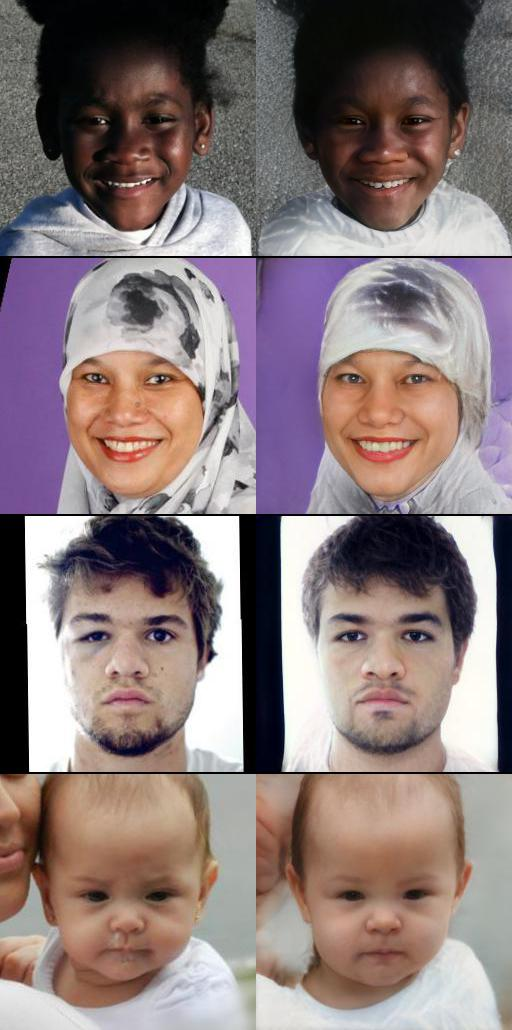
\includegraphics[width=0.7\textwidth]{figures/fair2fake.jpg}
    \captionof{figure}{Selected FairFace images before/after encoding by pixel2style2pixel}
    \label{fair2fake}
  \end{Figure}

  \subsection{Model Performance Results}

  The baseline model achieved the following performance on the Fake Faces test
  set, after 18 training epochs (Table \ref{baseline-metrics}):

  \begin{Figure}
    \captionof{table}{Baseline model performance}
    \label{baseline-metrics}
    \begin{tabular}{rrrr}
    \toprule
     Accuracy &        F1 &  Precision &    Recall \\
    \midrule
     0.942197 &  0.941569 &   0.951865 &  0.931493 \\
    \bottomrule
    \end{tabular}
  \end{Figure}

  Our best model in hyperparameter tuning was a variant of the VGG architecture
  \cite{simonyan2015deep} with 10 total layers (8 convolution layers and 2 fully
  connected layers). This model's performance is given by
  (Figure \ref{vgg10-fakeface-metrics}).

  \begin{Figure}
    \centering
    \captionof{table}{Model performance on Fake Faces test set}
    \label{vgg10-fakeface-metrics}
    \begin{tabular}{rrrr}
    \toprule
     Accuracy &        F1 &  Precision &    Recall \\
    \midrule
     0.968298 &  0.967689 &   0.986595 &  0.949495 \\
    \bottomrule
    \end{tabular}
  \end{Figure}


  \subsection{Fairness Assessment Results}

  Our best model trained on the 70k real and fake faces dataset failed to
  generalize to the FairFace dataset, marking nearly all of the FairFace
  observations as fake faces, resulting in high recall but very low precision
  and accuracy scores (Figure \ref{vgg10-transfer-fail}).

  \begin{Figure}
    \centering
    \captionof{table}{Model performance metrics}
    \label{vgg10-transfer-fail}
    \begin{tabular}{rrrr}
    \toprule
    Accuracy &        F1 &  Precision &  Recall \\
    \midrule
      0.54305 &  0.676667 &    0.52357 &  0.9563 \\
    \bottomrule
    \end{tabular}
  \end{Figure}

  We originally intended to perform a fairness assessment on both our baseline
  model and our best model trained on the fake faces dataset, but because
  these models completely failed to generalize to the FairFace data,
  we decided not to even assess their demographic fairness metrics. Rather, we
  retrained our best model on a combined dataset consisting of the entire
  training sets from both the 70k real and fake faces and the FairFace datasets.

  The resulting model performed very well on the combined dataset (Figure
  \ref{vgg10-combined-metrics}), and even performed better on the 70 real and
  fake faces dataset than the model version that was only trained on that
  dataset (Figure \ref{vgg10-combined-fakefaces-metrics}), suggesting that the
  additional training examples from FairFace led to a general improvement.

  \begin{Figure}
    \centering
    \captionof{table}{Model performance metrics on FairFace + Fake Faces combined dataset}
    \label{vgg10-combined-metrics}
    \begin{tabular}{rrrr}
    \toprule
    Accuracy &        F1 &  Precision &    Recall \\
    \midrule
    0.984457 &  0.984411 &   0.986268 &  0.982561 \\
    \bottomrule
    \end{tabular}
  \end{Figure}

  \begin{Figure}
    \centering
    \captionof{table}{Performance on Fake Faces test set for model trained on combined dataset}
    \label{vgg10-combined-fakefaces-metrics}
    \begin{tabular}{rrrr}
    \toprule
     Accuracy &        F1 &  Precision &    Recall \\
    \midrule
     0.971232 &  0.971092 &    0.97374 &  0.968458 \\
    \bottomrule
    \end{tabular}
    \end{Figure}

  Our best model, using the VGG10 architecture and trained on the combined
  dataset, achieved excellent performance by the fairness metrics, disparate
  impact ratio (where 1.0 is perfectly fair) and average odds difference
  (where 0.0 is perfectly fair).

    \begin{Figure}
      \centering
      \captionof{table}{Model Fairness metrics}
      \label{fairnessmetrics}
      \begin{tabular}{lrr}
      \toprule
      {} &  Disparate Impact &  Avg Odds Diff \\
      \midrule
      Male       &                0.993955 &                -0.000031 \\
      White      &                1.027800 &                -0.001012 \\
      Non-Black  &                1.004817 &                 0.000983 \\
      Non-Child  &                1.011344 &                 0.000167 \\
      Non-Senior &                1.003951 &                 0.001968 \\
      \bottomrule
      \end{tabular}
      \end{Figure}

  \section{Discussion}
  Our initial goal of detecting fake faces was quite successful, especially on
  the original dataset. The <Insert finalized model name> managed an accuarcy of
  <x> percent when testing with the initial dataset. After some thorough testing
  and investigation, we made the decision to incorporate other fake images, and
  to go as far as making it more fair.

  After a successfully testing our network against same set testing images, we
  thought that our model was doing quite well so we moved onto external
  datasets. Upon testing with other fake images, we noted that the accuracy took
  a dramatic turn in the opposite direction. While investigating, we determined
  that there could be several causes for this decrease:

  \begin{enumerate}
    \tightlist
  		\item The original training set had a specific pattern the our models were
  		detecting, causing our network to look for those specific details. It
  		could be something minute, such as the eyes having x and y coordinates
  		that were within a specific range. Although, we deteremined that this was
  		unlikely due to our randomness when pre-processing (add noise, flips,
  		shears, rotations) our data.
  		\item Our method for creating a fair face dataset was flawed <talk about
  		how we got this dataset>
  		\item We didn't have enough data in original dataset to allow for a higher
  		classification rate outside of that set.
	\end{enumerate}

  \subsection{Future Work}
  Overall, we are quite happy with the way our model classifies, but there are
  several adjustments we'd love to make that could help increase accuracy. We do
  not believe that there were any fundamental flaws in our methods, rather an
  inadequate amount of time, resources, and overall data. All of issues revolve
  around a lack of time, and given more, we could increase the performance of
  our model architecture and classification.

  Time was our largest blocker throughout the entirety of our project, whether
  it was the time required to set up CUDA, train, or research new theories.
  During our models training time, we never saw a hint at over fitting, which
  indicated that there was still performance to be had. Given more time and
  compute power, we could have increased our accuracy. In addition, we could
  also take some images from NVIDA's fake face dataset and add that to our
  training data, but once again the cost involved is more than our team could
  handle.

  In the future, we would love to incorporate these changes and throw more
  compute power at the problem. Using ample amounts of training data and more
  computer vision techniques we believe that there is still room to improve on
  our model. Although, as fake faces become better in better, we wonder how our
  model would fare. Looking at a company like NVIDIA, who has the resources to
  make fake faces using GANNs and enormous amounts of compute power, will it be
  possible to detect their fake faces?

\end{multicols}

\bibliography{report}
\bibliographystyle{unsrt}
\end{document}
